\documentclass[11pt, a4paper]{article}

% Fonts and Encoding
\usepackage[utf8]{inputenc}
\usepackage[T1]{fontenc}
\usepackage{lmodern}

% Math and Symbols
\usepackage{amsmath, amssymb, amsthm, amsfonts, mathrsfs, mathtools}

% Layout and Geometry
\usepackage{geometry}
\geometry{a4paper, margin=1in}

% Formatting and Graphics
\usepackage{graphicx, xcolor, enumitem, booktabs, array, tabularx}

% TikZ for Illustrations
\usepackage{tikz}
\usetikzlibrary{arrows.meta, positioning, shapes.geometric, calc, backgrounds, matrix}

% Clickable Links and TOC
\usepackage{hyperref}
\hypersetup{
    colorlinks=true,
    linkcolor=blue,
    filecolor=magenta,      
    urlcolor=cyan,
    pdftitle={Eigenvalues and Eigenvectors},
}

% Theorem Environments
\newtheorem{theorem}{Theorem}[section]
\newtheorem{lemma}[theorem]{Lemma}
\newtheorem{proposition}[theorem]{Proposition}
\newtheorem{corollary}[theorem]{Corollary}
\theoremstyle{definition}
\newtheorem{definition}{Definition}[section]
\newtheorem{axiom}{Axiom}[section]
\newtheorem{example}{Example}[section]
\theoremstyle{remark}
\newtheorem{remark}{Remark}[section]

% Custom Commands (Enforced standard notation)
\newcommand{\R}{\mathbb{R}}
\newcommand{\N}{\mathbb{N}}
\newcommand{\Z}{\mathbb{Z}}
\newcommand{\Q}{\mathbb{Q}}
\newcommand{\E}{\mathbb{E}}
\newcommand{\Prob}{\mathbb{P}}
\newcommand{\F}{\mathcal{F}}

\begin{document}

\title{\textbf{Mastering Linear Algebra: Eigenvalues and Eigenvectors}}
\author{Tashfeen Omran}
\date{\today}

\maketitle
\tableofcontents
\newpage

\section{Part 1: Comprehensive Introduction, Context, and Prerequisites}

\subsection{Core Concepts}
The study of \textbf{Eigenvalues and Eigenvectors} is fundamentally about understanding the invariant properties of linear transformations. When a square matrix $A$ multiplies a vector $\mathbf{x}$, the resulting vector $A\mathbf{x}$ is generally transformed in both magnitude and direction. However, for any given matrix $A$, there often exist special vectors whose \textit{direction} is perfectly preserved (or exactly reversed) by the transformation. 

For these special vectors, the action of matrix multiplication simplifies to mere scalar multiplication. We define an \textbf{eigenvector} of an $n \times n$ matrix $A$ as a \textit{nonzero} vector $\mathbf{x}$ such that:
\[ A\mathbf{x} = \lambda \mathbf{x} \]
where $\lambda$ is a scalar known as the \textbf{eigenvalue} corresponding to $\mathbf{x}$. The set of all eigenvectors corresponding to a specific eigenvalue $\lambda$, together with the zero vector, forms a subspace of $\R^n$ called the \textbf{eigenspace}.

\subsection{Intuition and Derivation}
Geometrically, if you consider a linear transformation as a stretching, squashing, or rotating of space, the eigenvectors are the "axes" of that transformation that do not get knocked off their span. The eigenvalue $\lambda$ measures the factor by which the eigenvector is stretched or compressed. If $\lambda$ is negative, the vector's direction is flipped.

Algebraically, the equation $A\mathbf{x} = \lambda \mathbf{x}$ can be rewritten by bringing all terms to one side:
\[ A\mathbf{x} - \lambda \mathbf{x} = \mathbf{0} \]
Factoring out $\mathbf{x}$ requires the use of the identity matrix $I$ (since we cannot subtract a scalar from a matrix):
\[ (A - \lambda I)\mathbf{x} = \mathbf{0} \]
For $\mathbf{x}$ to be a \textit{nonzero} eigenvector, the matrix $(A - \lambda I)$ must not be invertible. If it were invertible, the only solution would be the trivial solution $\mathbf{x} = \mathbf{0}$. Therefore, the null space of $(A - \lambda I)$ must be non-trivial, which is the foundational mechanism for finding eigenspaces.

\subsection{Historical Context and Motivation}
The concepts of eigenvalues and eigenvectors originated in the 18th century through the study of rigid body dynamics and celestial mechanics. Mathematicians like Leonhard Euler and Joseph-Louis Lagrange were trying to find the "principal axes" of rotating bodies—axes about which a body could rotate without wobbling. Later, Augustin-Louis Cauchy formalized these ideas while studying quadratic forms and the stress tensor in elasticity theory. The term "eigen" comes from German, meaning "proper," "characteristic," or "own," highlighting that these vectors are intrinsic properties of the matrix itself.

\subsection{Key Formulas}
\begin{itemize}
    \item \textbf{The Eigenvalue Equation:} $A\mathbf{x} = \lambda \mathbf{x}$ (where $\mathbf{x} \neq \mathbf{0}$).
    \item \textbf{The Homogeneous System for Eigenspaces:} $(A - \lambda I)\mathbf{x} = \mathbf{0}$.
    \item \textbf{The Characteristic Equation:} $\det(A - \lambda I) = 0$ (used to find eigenvalues, though heavily explored in subsequent sections).
\end{itemize}

\subsection{Prerequisites}
To master this topic, you must be fluent in:
\begin{itemize}
    \item \textbf{Matrix Multiplication:} Computing $A\mathbf{x}$.
    \item \textbf{Row Reduction (Gaussian Elimination):} Reducing augmented matrices to Reduced Row Echelon Form (RREF).
    \item \textbf{Null Spaces:} Finding the parametric vector form of solutions to homogeneous systems $B\mathbf{x} = \mathbf{0}$.
    \item \textbf{Linear Independence:} Understanding when a set of vectors forms a basis for a subspace.
\end{itemize}

\newpage
\section{Part 2: Detailed Homework Solutions}
\textit{Note: Per the strategic selection protocol, we have selected a representative sample of problems that covers every distinct archetype present in the provided text, ensuring comprehensive mastery without redundant repetition.}

\subsection{Problem 1: Verifying an Eigenvalue}
\textbf{Question:} Is $\lambda = 2$ an eigenvalue of $A = \begin{bmatrix} 3 & 2 \\ 3 & 8 \end{bmatrix}$? Why or why not?

\textbf{Solution:}
We must determine if the equation $(A - 2I)\mathbf{x} = \mathbf{0}$ has a nontrivial solution. First, we construct the matrix $A - 2I$:
\[
A - 2I = \begin{bmatrix} 3 & 2 \\ 3 & 8 \end{bmatrix} - \begin{bmatrix} 2 & 0 \\ 0 & 2 \end{bmatrix} = \begin{bmatrix} 1 & 2 \\ 3 & 6 \end{bmatrix}
\]
Next, we row reduce the augmented matrix for the homogeneous system:
\[
\begin{bmatrix} 1 & 2 & 0 \\ 3 & 6 & 0 \end{bmatrix}
\]
Apply the row operation $R_2 \leftarrow R_2 - 3R_1$:
\[
\begin{bmatrix} 1 & 2 & 0 \\ 0 & 0 & 0 \end{bmatrix}
\]
The system has a free variable ($x_2$), which means there are infinitely many nontrivial solutions. 
\textbf{Final Answer:} Yes, $\lambda = 2$ is an eigenvalue because $(A - 2I)\mathbf{x} = \mathbf{0}$ has a nontrivial solution.

\subsection{Problem 7: Verifying an Eigenvalue (3x3)}
\textbf{Question:} Is $\lambda = 4$ an eigenvalue of $A = \begin{bmatrix} 3 & 0 & -1 \\ 2 & 3 & 1 \\ -3 & 4 & 5 \end{bmatrix}$? If so, find one corresponding eigenvector.

\textbf{Solution:}
Construct $A - 4I$:
\[
A - 4I = \begin{bmatrix} 3-4 & 0 & -1 \\ 2 & 3-4 & 1 \\ -3 & 4 & 5-4 \end{bmatrix} = \begin{bmatrix} -1 & 0 & -1 \\ 2 & -1 & 1 \\ -3 & 4 & 1 \end{bmatrix}
\]
Row reduce the augmented matrix:
\[
\begin{bmatrix} -1 & 0 & -1 & 0 \\ 2 & -1 & 1 & 0 \\ -3 & 4 & 1 & 0 \end{bmatrix}
\]
$R_2 \leftarrow R_2 + 2R_1$ and $R_3 \leftarrow R_3 - 3R_1$:
\[
\begin{bmatrix} -1 & 0 & -1 & 0 \\ 0 & -1 & -1 & 0 \\ 0 & 4 & 4 & 0 \end{bmatrix}
\]
$R_3 \leftarrow R_3 + 4R_2$:
\[
\begin{bmatrix} -1 & 0 & -1 & 0 \\ 0 & -1 & -1 & 0 \\ 0 & 0 & 0 & 0 \end{bmatrix}
\]
Multiply $R_1$ and $R_2$ by $-1$:
\[
\begin{bmatrix} 1 & 0 & 1 & 0 \\ 0 & 1 & 1 & 0 \\ 0 & 0 & 0 & 0 \end{bmatrix}
\]
The equations are $x_1 + x_3 = 0$ and $x_2 + x_3 = 0$. Thus, $x_1 = -x_3$ and $x_2 = -x_3$. Let $x_3 = 1$.
\textbf{Final Answer:} Yes, $\lambda = 4$ is an eigenvalue. A corresponding eigenvector is $\begin{bmatrix} -1 \\ -1 \\ 1 \end{bmatrix}$.

\subsection{Problem 3: Verifying an Eigenvector}
\textbf{Question:} Is $\begin{bmatrix} 1 \\ 4 \end{bmatrix}$ an eigenvector of $\begin{bmatrix} -3 & 1 \\ -3 & 8 \end{bmatrix}$? If so, find the eigenvalue.

\textbf{Solution:}
Let $A = \begin{bmatrix} -3 & 1 \\ -3 & 8 \end{bmatrix}$ and $\mathbf{v} = \begin{bmatrix} 1 \\ 4 \end{bmatrix}$. We compute $A\mathbf{v}$:
\[
A\mathbf{v} = \begin{bmatrix} -3 & 1 \\ -3 & 8 \end{bmatrix} \begin{bmatrix} 1 \\ 4 \end{bmatrix} = \begin{bmatrix} -3(1) + 1(4) \\ -3(1) + 8(4) \end{bmatrix} = \begin{bmatrix} 1 \\ 29 \end{bmatrix}
\]
We must check if $A\mathbf{v}$ is a scalar multiple of $\mathbf{v}$. Is there a scalar $\lambda$ such that $\begin{bmatrix} 1 \\ 29 \end{bmatrix} = \lambda \begin{bmatrix} 1 \\ 4 \end{bmatrix}$?
For the first component, $\lambda = 1$. For the second component, $4\lambda = 29 \implies \lambda = 7.25$. Since the scalar is not consistent, $A\mathbf{v}$ is not a multiple of $\mathbf{v}$.
\textbf{Final Answer:} No, it is not an eigenvector.

\subsection{Problem 5: Verifying an Eigenvector with Zero Eigenvalue}
\textbf{Question:} Is $\begin{bmatrix} 4 \\ -3 \\ 1 \end{bmatrix}$ an eigenvector of $\begin{bmatrix} 3 & 7 & 9 \\ -4 & -5 & 1 \\ 2 & 4 & 4 \end{bmatrix}$? If so, find the eigenvalue.

\textbf{Solution:}
Let $A$ be the given matrix and $\mathbf{v}$ be the vector. Compute $A\mathbf{v}$:
\[
A\mathbf{v} = \begin{bmatrix} 3 & 7 & 9 \\ -4 & -5 & 1 \\ 2 & 4 & 4 \end{bmatrix} \begin{bmatrix} 4 \\ -3 \\ 1 \end{bmatrix} = \begin{bmatrix} 3(4) + 7(-3) + 9(1) \\ -4(4) - 5(-3) + 1(1) \\ 2(4) + 4(-3) + 4(1) \end{bmatrix} = \begin{bmatrix} 12 - 21 + 9 \\ -16 + 15 + 1 \\ 8 - 12 + 4 \end{bmatrix} = \begin{bmatrix} 0 \\ 0 \\ 0 \end{bmatrix}
\]
We can write this as $A\mathbf{v} = 0 \cdot \mathbf{v}$. Since $\mathbf{v}$ is a nonzero vector and satisfies $A\mathbf{v} = \lambda \mathbf{v}$ for $\lambda = 0$, it is an eigenvector.
\textbf{Final Answer:} Yes, it is an eigenvector, and the corresponding eigenvalue is $\lambda = 0$.

\subsection{Problem 9: Finding a Basis for an Eigenspace}
\textbf{Question:} Find a basis for the eigenspace corresponding to $\lambda = 3, 9$ for $A = \begin{bmatrix} 9 & 0 \\ 2 & 3 \end{bmatrix}$.

\textbf{Solution:}
\textbf{Case 1: $\lambda = 3$}
Construct $A - 3I$:
\[
A - 3I = \begin{bmatrix} 6 & 0 \\ 2 & 0 \end{bmatrix}
\]
Row reduce $(A - 3I)\mathbf{x} = \mathbf{0}$:
\[
\begin{bmatrix} 6 & 0 & 0 \\ 2 & 0 & 0 \end{bmatrix} \sim \begin{bmatrix} 1 & 0 & 0 \\ 0 & 0 & 0 \end{bmatrix}
\]
This gives $x_1 = 0$, and $x_2$ is free. The parametric vector form is $\mathbf{x} = x_2 \begin{bmatrix} 0 \\ 1 \end{bmatrix}$.
Basis for $\lambda = 3$: $\left\{ \begin{bmatrix} 0 \\ 1 \end{bmatrix} \right\}$.

\textbf{Case 2: $\lambda = 9$}
Construct $A - 9I$:
\[
A - 9I = \begin{bmatrix} 0 & 0 \\ 2 & -6 \end{bmatrix}
\]
Row reduce $(A - 9I)\mathbf{x} = \mathbf{0}$:
\[
\begin{bmatrix} 0 & 0 & 0 \\ 2 & -6 & 0 \end{bmatrix} \sim \begin{bmatrix} 1 & -3 & 0 \\ 0 & 0 & 0 \end{bmatrix}
\]
This gives $x_1 - 3x_2 = 0 \implies x_1 = 3x_2$, and $x_2$ is free. The parametric vector form is $\mathbf{x} = x_2 \begin{bmatrix} 3 \\ 1 \end{bmatrix}$.
\textbf{Final Answer:} Basis for $\lambda = 3$ is $\left\{ \begin{bmatrix} 0 \\ 1 \end{bmatrix} \right\}$. Basis for $\lambda = 9$ is $\left\{ \begin{bmatrix} 3 \\ 1 \end{bmatrix} \right\}$.

\subsection{Problem 13: Finding Bases for Multiple Eigenspaces}
\textbf{Question:} Find a basis for the eigenspaces of $A = \begin{bmatrix} 4 & 0 & 1 \\ -2 & 1 & 0 \\ -2 & 0 & 1 \end{bmatrix}$ corresponding to $\lambda = 1, 2, 3$.

\textbf{Solution:}
\textbf{For $\lambda = 1$:}
\[
A - 1I = \begin{bmatrix} 3 & 0 & 1 \\ -2 & 0 & 0 \\ -2 & 0 & 0 \end{bmatrix} \sim \begin{bmatrix} 1 & 0 & 0 \\ 0 & 0 & 1 \\ 0 & 0 & 0 \end{bmatrix}
\]
Equations: $x_1 = 0$, $x_3 = 0$, $x_2$ is free. Basis: $\left\{ \begin{bmatrix} 0 \\ 1 \\ 0 \end{bmatrix} \right\}$.

\textbf{For $\lambda = 2$:}
\[
A - 2I = \begin{bmatrix} 2 & 0 & 1 \\ -2 & -1 & 0 \\ -2 & 0 & -1 \end{bmatrix}
\]
$R_2 \leftarrow R_2 + R_1$ and $R_3 \leftarrow R_3 + R_1$:
\[
\begin{bmatrix} 2 & 0 & 1 \\ 0 & -1 & 1 \\ 0 & 0 & 0 \end{bmatrix} \sim \begin{bmatrix} 1 & 0 & 1/2 \\ 0 & 1 & -1 \\ 0 & 0 & 0 \end{bmatrix}
\]
Equations: $x_1 = -\frac{1}{2}x_3$, $x_2 = x_3$. Let $x_3 = 2$ to clear fractions. Basis: $\left\{ \begin{bmatrix} -1 \\ 2 \\ 2 \end{bmatrix} \right\}$.

\textbf{For $\lambda = 3$:}
\[
A - 3I = \begin{bmatrix} 1 & 0 & 1 \\ -2 & -2 & 0 \\ -2 & 0 & -2 \end{bmatrix}
\]
$R_2 \leftarrow R_2 + 2R_1$ and $R_3 \leftarrow R_3 + 2R_1$:
\[
\begin{bmatrix} 1 & 0 & 1 \\ 0 & -2 & 2 \\ 0 & 0 & 0 \end{bmatrix} \sim \begin{bmatrix} 1 & 0 & 1 \\ 0 & 1 & -1 \\ 0 & 0 & 0 \end{bmatrix}
\]
Equations: $x_1 = -x_3$, $x_2 = x_3$. Let $x_3 = 1$. Basis: $\left\{ \begin{bmatrix} -1 \\ 1 \\ 1 \end{bmatrix} \right\}$.

\textbf{Final Answer:} The bases are $\left\{ \begin{bmatrix} 0 \\ 1 \\ 0 \end{bmatrix} \right\}$ for $\lambda=1$, $\left\{ \begin{bmatrix} -1 \\ 2 \\ 2 \end{bmatrix} \right\}$ for $\lambda=2$, and $\left\{ \begin{bmatrix} -1 \\ 1 \\ 1 \end{bmatrix} \right\}$ for $\lambda=3$.

\subsection{Problem 17: Eigenvalues of a Triangular Matrix}
\textbf{Question:} Find the eigenvalues of $A = \begin{bmatrix} 0 & 0 & 0 \\ 0 & 2 & 5 \\ 0 & 0 & -1 \end{bmatrix}$.

\textbf{Solution:}
By Theorem 1 in the text, the eigenvalues of a triangular matrix are the entries on its main diagonal. The given matrix is upper triangular because all entries below the main diagonal are zero.
\textbf{Final Answer:} The eigenvalues are $\lambda = 0, 2, -1$.

\subsection{Problem 31: Conceptual Proof}
\textbf{Question:} Explain why a $2 \times 2$ matrix can have at most two distinct eigenvalues. Explain why an $n \times n$ matrix can have at most $n$ distinct eigenvalues.

\textbf{Solution:}
By Theorem 2, eigenvectors corresponding to distinct eigenvalues are linearly independent. If an $n \times n$ matrix had more than $n$ distinct eigenvalues, it would possess more than $n$ linearly independent eigenvectors. However, any set of more than $n$ vectors in $\R^n$ is linearly dependent. This creates a contradiction. Therefore, an $n \times n$ matrix can have at most $n$ distinct eigenvalues. (Consequently, a $2 \times 2$ matrix can have at most 2).

\subsection{Problem 33: Abstract Properties}
\textbf{Question:} Let $\lambda$ be an eigenvalue of an invertible matrix $A$. Show that $\lambda^{-1}$ is an eigenvalue of $A^{-1}$.

\textbf{Solution:}
Since $\lambda$ is an eigenvalue of $A$, there exists a nonzero vector $\mathbf{x}$ such that:
\[ A\mathbf{x} = \lambda \mathbf{x} \]
Because $A$ is invertible, its null space contains only the zero vector, meaning $0$ cannot be an eigenvalue of $A$. Thus, $\lambda \neq 0$. We can multiply both sides of the equation on the left by $A^{-1}$:
\[ A^{-1}(A\mathbf{x}) = A^{-1}(\lambda \mathbf{x}) \]
\[ (A^{-1}A)\mathbf{x} = \lambda (A^{-1}\mathbf{x}) \]
\[ I\mathbf{x} = \lambda A^{-1}\mathbf{x} \]
\[ \mathbf{x} = \lambda A^{-1}\mathbf{x} \]
Since $\lambda \neq 0$, we can divide both sides by $\lambda$:
\[ \frac{1}{\lambda}\mathbf{x} = A^{-1}\mathbf{x} \]
Rearranging yields $A^{-1}\mathbf{x} = \lambda^{-1}\mathbf{x}$. Since $\mathbf{x}$ is nonzero, this proves that $\lambda^{-1}$ is an eigenvalue of $A^{-1}$.

\newpage
\section{Part 3: In-Depth Analysis of Problems and Techniques}

\subsection{A) Problem Types and General Approach}
The homework problems can be categorized into three distinct archetypes:

1. \textbf{Verification Problems (e.g., Problems 1, 3, 5, 7):}
   \begin{itemize}
       \item \textit{Strategy for Eigenvectors:} Multiply the given matrix $A$ by the given vector $\mathbf{v}$. Check if the resulting vector $A\mathbf{v}$ is a scalar multiple of $\mathbf{v}$. If $A\mathbf{v} = \lambda \mathbf{v}$, it is an eigenvector.
       \item \textit{Strategy for Eigenvalues:} Subtract $\lambda I$ from $A$. Row reduce the resulting matrix to see if there is a free variable. If a free variable exists, the null space is non-trivial, confirming $\lambda$ is an eigenvalue.
   \end{itemize}

2. \textbf{Eigenspace Extraction Problems (e.g., Problems 9, 13):}
   \begin{itemize}
       \item \textit{Strategy:} Given an eigenvalue $\lambda$, compute the matrix $A - \lambda I$. Set up the homogeneous system $(A - \lambda I)\mathbf{x} = \mathbf{0}$ and row reduce to RREF. Express the basic variables in terms of the free variables to write the solution in parametric vector form. The vectors attached to the free variables form the basis for the eigenspace.
   \end{itemize}

3. \textbf{Theoretical and Abstract Problems (e.g., Problems 17, 31, 33):}
   \begin{itemize}
       \item \textit{Strategy:} Rely on established theorems rather than brute-force computation. For triangular matrices, read the diagonal. For proofs involving inverses or powers of matrices, start with the foundational definition $A\mathbf{x} = \lambda \mathbf{x}$ and apply matrix algebra (multiplying by inverses, factoring) to manipulate the equation into the desired form.
   \end{itemize}

\subsection{B) Key Algebraic and Calculus Manipulations}

\renewcommand{\arraystretch}{1.5}
\noindent
\begin{tabularx}{\textwidth}{lX}
\toprule
\textbf{Technique} & \textbf{Application and Example from Homework} \\
\midrule
\textbf{Matrix Shifting} & 
Subtracting $\lambda$ from the main diagonal of $A$ to form $A - \lambda I$. This algebraic trick converts the eigenvalue problem $A\mathbf{x} = \lambda \mathbf{x}$ into a null space problem $(A - \lambda I)\mathbf{x} = \mathbf{0}$. Used extensively in Problems 1, 7, 9, and 13. \\
\addlinespace[4pt]
\textbf{Parametric Vector Form} & 
Extracting a basis from RREF. In Problem 13, the equation $x_1 + \frac{1}{2}x_3 = 0$ was manipulated to $x_1 = -\frac{1}{2}x_3$. Factoring out the free variable $x_3$ isolates the basis vector. \\
\addlinespace[4pt]
\textbf{Fraction Clearing} & 
Because any scalar multiple of an eigenvector is still an eigenvector, we can scale basis vectors to remove fractions. In Problem 13, the vector $\displaystyle \begin{bmatrix} -1/2 \\ 1 \\ 1 \end{bmatrix}$ was multiplied by 2 to yield the cleaner basis vector $\displaystyle \begin{bmatrix} -1 \\ 2 \\ 2 \end{bmatrix}$. \\
\addlinespace[4pt]
\textbf{Left-Multiplication} & 
In Problem 33, proving properties of $A^{-1}$ required left-multiplying the equation $A\mathbf{x} = \lambda \mathbf{x}$ by $A^{-1}$. Matrix multiplication is not commutative, so maintaining strict left-multiplication order is a critical algebraic mandate. \\
\bottomrule
\end{tabularx}

\newpage
\section{Part 4: "Cheatsheet" and Tips for Success}

\subsection{Summary of Important Formulas}
\renewcommand{\arraystretch}{1.5}
\noindent
\begin{tabularx}{\textwidth}{lX}
\toprule
\textbf{Concept} & \textbf{Formula / Definition} \\
\midrule
\textbf{Eigenvector Definition} & $\displaystyle A\mathbf{x} = \lambda \mathbf{x} \quad (\text{where } \mathbf{x} \neq \mathbf{0})$ \\
\textbf{Eigenspace Equation} & $\displaystyle (A - \lambda I)\mathbf{x} = \mathbf{0}$ \\
\textbf{Triangular Matrix Theorem} & If $A$ is upper or lower triangular, the eigenvalues are exactly the entries $a_{11}, a_{22}, \dots, a_{nn}$ on the main diagonal. \\
\bottomrule
\end{tabularx}

\subsection{Tricks, Shortcuts, and Visualizations}
\begin{itemize}
    \item \textbf{The Triangular Shortcut:} Never row reduce a triangular matrix to find its eigenvalues. Just read them off the diagonal.
    \item \textbf{The Zero Eigenvalue Check:} A matrix has an eigenvalue of $0$ if and only if it is \textit{not} invertible (i.e., its determinant is zero, or it has free variables).
    \item \textbf{Scaling Eigenvectors:} If you find an eigenvector with messy fractions, multiply it by the least common denominator. The eigenspace is a line (or plane), so any scaled version of the vector is equally valid.
\end{itemize}

\begin{figure}[h!]
\centering
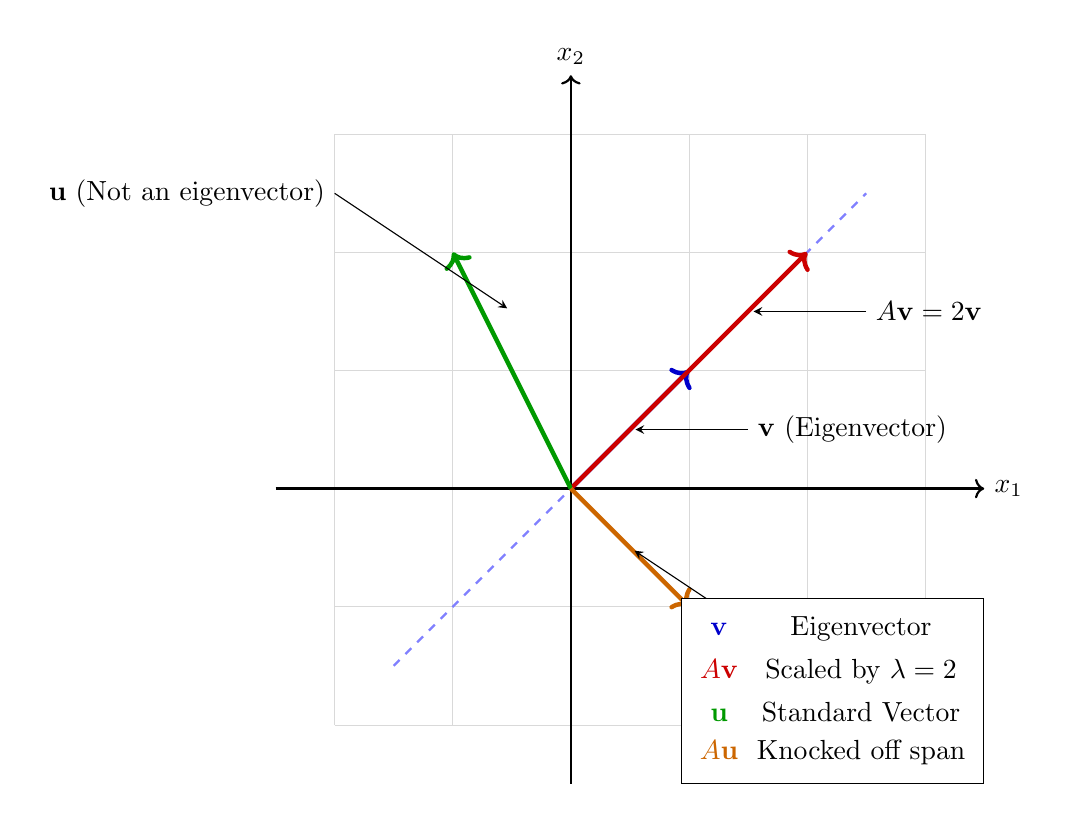
\begin{tikzpicture}[scale=1.5, background rectangle/.style={fill=white}, show background rectangle]
    % Grid and Axes
    \draw[step=1cm, gray!30, very thin] (-2,-2) grid (3,3);
    \draw[thick, ->] (-2.5,0) -- (3.5,0) node[right, text=black] {$x_1$};
    \draw[thick, ->] (0,-2.5) -- (0,3.5) node[above, text=black] {$x_2$};

    % Eigenspace Line
    \draw[dashed, blue!50, thick] (-1.5,-1.5) -- (2.5,2.5);

    % Eigenvector v
    \draw[->, ultra thick, blue!80!black] (0,0) -- (1,1);
    \draw[->, >=stealth, shorten >=2pt] (1.5, 0.5) -- (0.5, 0.5);
    \node[right, text=black] at (1.5, 0.5) {$\displaystyle \mathbf{v}$ (Eigenvector)};

    % Transformed Eigenvector Av
    \draw[->, ultra thick, red!80!black] (0,0) -- (2,2);
    \draw[->, >=stealth, shorten >=2pt] (2.5, 1.5) -- (1.5, 1.5);
    \node[right, text=black] at (2.5, 1.5) {$\displaystyle A\mathbf{v} = 2\mathbf{v}$};

    % Non-Eigenvector u
    \draw[->, ultra thick, green!60!black] (0,0) -- (-1,2);
    \draw[->, >=stealth, shorten >=2pt] (-2, 2.5) -- (-0.5, 1.5);
    \node[left, text=black] at (-2, 2.5) {$\displaystyle \mathbf{u}$ (Not an eigenvector)};

    % Transformed Non-Eigenvector Au
    \draw[->, ultra thick, orange!80!black] (0,0) -- (1,-1);
    \draw[->, >=stealth, shorten >=2pt] (2, -1.5) -- (0.5, -0.5);
    \node[right, text=black] at (2, -1.5) {$\displaystyle A\mathbf{u}$ (Off-axis)};

    % Legend
    \matrix [matrix of nodes, draw, fill=white, anchor=south east] at (3.5, -2.5) {
        |[text=blue!80!black]| $\mathbf{v}$ & |[text=black]| Eigenvector \\
        |[text=red!80!black]| $A\mathbf{v}$ & |[text=black]| Scaled by $\lambda=2$ \\
        |[text=green!60!black]| $\mathbf{u}$ & |[text=black]| Standard Vector \\
        |[text=orange!80!black]| $A\mathbf{u}$ & |[text=black]| Knocked off span \\
    };
\end{tikzpicture}
\caption{Geometric interpretation of eigenvectors. The vector $\mathbf{v}$ remains on its original span (the dashed line) after transformation, whereas $\mathbf{u}$ is rotated away from its original span.}
\end{figure}

\subsection{Common Pitfalls and Traps}
\begin{itemize}
    \item \textbf{The Zero Vector Trap:} The zero vector $\mathbf{0}$ is \textit{never} an eigenvector, by definition. However, the scalar $0$ \textit{can} be an eigenvalue.
    \item \textbf{Row Reducing $A$ Instead of $A - \lambda I$:} Row operations change the eigenvalues of a matrix! Never row reduce $A$ to find its eigenvalues. You only row reduce $A - \lambda I$ to find the eigenvectors.
    \item \textbf{Sign Errors in $A - \lambda I$:} When subtracting $\lambda$ from the diagonal, students often forget to distribute negative signs if the diagonal entry is already negative. Always write out the subtraction explicitly.
\end{itemize}

\newpage
\section{Part 5: Conceptual Synthesis and The "Big Picture"}

\subsection{A) Thematic Connections}
The central theme of eigenvalues and eigenvectors is \textbf{decoupling complex systems into independent, simpler components}. In earlier calculus, we approximated complex curves using linear tangent lines. In linear algebra, we approximate complex multidimensional transformations by finding the specific 1D lines (eigenspaces) where the transformation acts merely as a 1D scalar multiplication. This theme of "finding the right perspective" (or basis) to make a problem trivial is ubiquitous in mathematics.

\subsection{B) Forward and Backward Links}
\textbf{Backward Links:} This topic relies heavily on the concept of the \textit{Null Space} and \textit{Linear Independence} from earlier chapters. Finding an eigenspace is literally just finding the null space of a shifted matrix $(A - \lambda I)$. 

\textbf{Forward Links:} Mastering this section is the absolute bedrock for:
\begin{itemize}
    \item \textbf{Diagonalization:} In the next sections, you will learn that if a matrix has enough linearly independent eigenvectors, it can be factored as $A = PDP^{-1}$, where $D$ is a diagonal matrix of eigenvalues. This makes computing massive matrix powers ($A^{100}$) computationally trivial.
    \item \textbf{Differential Equations:} Systems of linear differential equations $\mathbf{x}'(t) = A\mathbf{x}(t)$ are solved by finding the eigenvalues of $A$. The eigenvalues dictate whether the system's state decays to zero, oscillates, or explodes to infinity.
    \item \textbf{Singular Value Decomposition (SVD):} The ultimate factorization of any matrix (even non-square ones) relies on the eigenvalues of $A^T A$.
\end{itemize}

\section{Part 6: Abstract Real-World Modeling (AI, ML, \& Quant Finance)}

\subsection{A) Concrete Scenarios}
\begin{enumerate}
    \item \textbf{Machine Learning (Principal Component Analysis):} In high-dimensional datasets (e.g., 10,000-pixel images), processing every feature is computationally impossible. PCA computes the covariance matrix of the data and finds its eigenvectors. The eigenvectors with the largest eigenvalues represent the "Principal Components"—the directions of maximum variance. We can compress the data by projecting it onto just these few eigenvectors.
    \item \textbf{Quantitative Finance (Portfolio Risk Management):} A covariance matrix is constructed representing the historical price correlations between hundreds of stocks. The eigenvectors of this matrix identify uncorrelated "risk factors" in the market, and the eigenvalues quantify the volatility of each factor. Quants use this to hedge portfolios against specific macro-economic risks.
    \item \textbf{Information Theory (Markov Chains \& PageRank):} Google's original PageRank algorithm models the internet as a massive transition matrix of probabilities. The "importance" of a webpage is determined by finding the steady-state vector of this matrix, which is mathematically just the eigenvector corresponding to the eigenvalue $\lambda = 1$.
\end{enumerate}

\subsection{B) Model Problem Setup: Principal Component Analysis (PCA)}
Let us rigorously formulate the PCA optimization problem. Suppose we have a centered dataset represented by a random vector $\mathbf{X} \in \R^n$ such that $\E[\mathbf{X}] = \mathbf{0}$. The covariance matrix is defined as $\Sigma = \E[\mathbf{X}\mathbf{X}^T]$, which is an $n \times n$ symmetric, positive semi-definite matrix.

We seek a normalized projection vector $\mathbf{w} \in \R^n$ (where $\|\mathbf{w}\|_2 = 1$) that maximizes the variance of the projected data. The variance of the projection is given by:
\[ \text{Var}(\mathbf{w}^T \mathbf{X}) = \E[(\mathbf{w}^T \mathbf{X})^2] = \E[\mathbf{w}^T \mathbf{X} \mathbf{X}^T \mathbf{w}] = \mathbf{w}^T \E[\mathbf{X}\mathbf{X}^T] \mathbf{w} = \mathbf{w}^T \Sigma \mathbf{w} \]

We formulate this as a constrained optimization problem:
\[ \max_{\mathbf{w}} \quad \mathbf{w}^T \Sigma \mathbf{w} \quad \text{subject to} \quad \mathbf{w}^T \mathbf{w} = 1 \]

To solve this, we introduce a Lagrange multiplier $\lambda$:
\[ \mathcal{L}(\mathbf{w}, \lambda) = \mathbf{w}^T \Sigma \mathbf{w} - \lambda(\mathbf{w}^T \mathbf{w} - 1) \]
Taking the gradient with respect to the vector $\mathbf{w}$ and setting it to zero:
\[ \nabla_{\mathbf{w}} \mathcal{L} = 2\Sigma \mathbf{w} - 2\lambda \mathbf{w} = \mathbf{0} \]
\[ \Sigma \mathbf{w} = \lambda \mathbf{w} \]
This is exactly the eigenvalue equation! The optimal projection direction $\mathbf{w}$ is the eigenvector of the covariance matrix $\Sigma$, and the maximum variance achieved is exactly the corresponding eigenvalue $\lambda$.

\newpage
\section{Part 7: Common Variations and Untested Concepts}

While the provided homework covers the mechanics of verifying and extracting eigenspaces, standard curriculums often test two additional concepts not heavily featured in this specific problem set.

\subsection{1. Complex Eigenvalues (Rotation Matrices)}
Not all real matrices have real eigenvalues. If a matrix represents a pure rotation in $\R^2$, it has no real eigenvectors because no vector maintains its original span.
\textbf{Example:} Find the eigenvalues of the $90^\circ$ rotation matrix $A = \begin{bmatrix} 0 & -1 \\ 1 & 0 \end{bmatrix}$.
\textbf{Solution:} We solve the characteristic equation $\det(A - \lambda I) = 0$:
\[ \det \begin{bmatrix} -\lambda & -1 \\ 1 & -\lambda \end{bmatrix} = (-\lambda)(-\lambda) - (-1)(1) = \lambda^2 + 1 = 0 \]
The roots are $\lambda = i$ and $\lambda = -i$. The lack of real eigenvalues perfectly matches the geometric intuition that a $90^\circ$ rotation leaves no real vector on its original axis.

\subsection{2. Algebraic vs. Geometric Multiplicity}
A critical concept for diagonalization is understanding multiplicities.
\begin{itemize}
    \item \textbf{Algebraic Multiplicity:} The number of times an eigenvalue appears as a root of the characteristic equation.
    \item \textbf{Geometric Multiplicity:} The dimension of the eigenspace corresponding to that eigenvalue (i.e., the number of free variables in $A - \lambda I$).
\end{itemize}
\textbf{Theorem:} The geometric multiplicity is always less than or equal to the algebraic multiplicity. If it is strictly less, the matrix is called "defective" and cannot be diagonalized.

\newpage
\section{Part 8: Advanced Diagnostic Testing: "Find the Flaw"}

\textit{Instructions: You are the grader. Each of the following five solutions contains a single, subtle conceptual or algebraic flaw. Identify the error in one sentence, then provide the correct step and final answer.}

\subsection{Problem 1}
\textbf{Question:} Find the eigenvalues of $A = \begin{bmatrix} 2 & 4 \\ 1 & 5 \end{bmatrix}$.
\textbf{Flawed Solution:} 
We row reduce matrix $A$ to find its eigenvalues.
$R_2 \leftarrow 2R_2 - R_1$: $\begin{bmatrix} 2 & 4 \\ 0 & 6 \end{bmatrix}$.
Since this is now an upper triangular matrix, the eigenvalues are the entries on the main diagonal. Therefore, $\lambda = 2$ and $\lambda = 6$.

\textbf{Grader's Correction:}
\begin{itemize}
    \item \textbf{The Flaw:} Row operations change the eigenvalues of a matrix, so you cannot row reduce $A$ before finding its eigenvalues.
    \item \textbf{Correct Step:} You must solve $\det(A - \lambda I) = 0$, which is $(2-\lambda)(5-\lambda) - 4 = \lambda^2 - 7\lambda + 6 = 0$.
    \item \textbf{Correct Answer:} Factoring yields $(\lambda - 6)(\lambda - 1) = 0$, so the true eigenvalues are $\lambda = 6$ and $\lambda = 1$.
\end{itemize}

\subsection{Problem 2}
\textbf{Question:} Is $\mathbf{v} = \begin{bmatrix} 0 \\ 0 \end{bmatrix}$ an eigenvector of $A = \begin{bmatrix} 3 & 1 \\ 0 & 2 \end{bmatrix}$?
\textbf{Flawed Solution:}
We multiply $A$ by $\mathbf{v}$:
$A\mathbf{v} = \begin{bmatrix} 3 & 1 \\ 0 & 2 \end{bmatrix} \begin{bmatrix} 0 \\ 0 \end{bmatrix} = \begin{bmatrix} 0 \\ 0 \end{bmatrix}$.
Since $A\mathbf{v} = 5 \cdot \mathbf{v}$ (or any scalar), the equation $A\mathbf{v} = \lambda \mathbf{v}$ holds true. Yes, it is an eigenvector.

\textbf{Grader's Correction:}
\begin{itemize}
    \item \textbf{The Flaw:} By strict mathematical definition, an eigenvector must be a nonzero vector.
    \item \textbf{Correct Step:} Recognize immediately that $\mathbf{v} = \mathbf{0}$.
    \item \textbf{Correct Answer:} No, the zero vector is never an eigenvector.
\end{itemize}

\subsection{Problem 3}
\textbf{Question:} Find a basis for the eigenspace of $A = \begin{bmatrix} 5 & -2 \\ 0 & 5 \end{bmatrix}$ corresponding to $\lambda = 5$.
\textbf{Flawed Solution:}
We construct $A - 5I = \begin{bmatrix} 0 & -2 \\ 0 & 0 \end{bmatrix}$.
This gives the equation $-2x_2 = 0$, so $x_2 = 0$. Since $x_2 = 0$, the only solution is the zero vector. Therefore, the matrix has no eigenvectors for $\lambda = 5$.

\textbf{Grader's Correction:}
\begin{itemize}
    \item \textbf{The Flaw:} The student failed to recognize that $x_1$ is a free variable because it does not have a pivot in the RREF matrix.
    \item \textbf{Correct Step:} With $x_2 = 0$ and $x_1$ free, the parametric vector form is $\mathbf{x} = x_1 \begin{bmatrix} 1 \\ 0 \end{bmatrix}$.
    \item \textbf{Correct Answer:} The basis for the eigenspace is $\left\{ \begin{bmatrix} 1 \\ 0 \end{bmatrix} \right\}$.
\end{itemize}

\subsection{Problem 4}
\textbf{Question:} If $A\mathbf{x} = \mathbf{0}$ for a nonzero vector $\mathbf{x}$, does $A$ have an eigenvalue?
\textbf{Flawed Solution:}
If $A\mathbf{x} = \mathbf{0}$, then the matrix transforms the vector into nothing. Because there is no scalar $\lambda$ stretching the vector, the matrix does not have an eigenvalue for this vector.

\textbf{Grader's Correction:}
\begin{itemize}
    \item \textbf{The Flaw:} The student incorrectly assumes that a scalar of zero means the eigenvalue does not exist.
    \item \textbf{Correct Step:} Rewrite $A\mathbf{x} = \mathbf{0}$ as $A\mathbf{x} = 0\mathbf{x}$.
    \item \textbf{Correct Answer:} Yes, $A$ has an eigenvalue, and that eigenvalue is exactly $\lambda = 0$.
\end{itemize}

\subsection{Problem 5}
\textbf{Question:} Find the eigenspace basis for $\lambda = 2$ given $A - 2I = \begin{bmatrix} 1 & -3 \\ 0 & 0 \end{bmatrix}$.
\textbf{Flawed Solution:}
The matrix gives the equation $x_1 - 3x_2 = 0$.
Solving for $x_1$, we get $x_1 = -3x_2$.
The parametric form is $\mathbf{x} = x_2 \begin{bmatrix} -3 \\ 1 \end{bmatrix}$. The basis is $\left\{ \begin{bmatrix} -3 \\ 1 \end{bmatrix} \right\}$.

\textbf{Grader's Correction:}
\begin{itemize}
    \item \textbf{The Flaw:} The student made a sign error when moving $-3x_2$ to the other side of the equation.
    \item \textbf{Correct Step:} $x_1 - 3x_2 = 0 \implies x_1 = 3x_2$.
    \item \textbf{Correct Answer:} The correct basis is $\left\{ \begin{bmatrix} 3 \\ 1 \end{bmatrix} \right\}$.
\end{itemize}

\end{document}